\section{Phân đoạn Ảnh (Image Segmentation)}
\label{sec:image_segmentation}

Trong khi phát hiện vật thể cung cấp câu trả lời "Cái gì?" và "Ở đâu?", bài toán phân đoạn ảnh tiến một bước sâu hơn về mặt chi tiết, nhằm trả lời câu hỏi \textbf{"Hình dạng chính xác của nó là gì?"}. Thay vì chỉ khoanh vùng đối tượng bằng một chiếc hộp chữ nhật thô, phân đoạn ảnh gán một nhãn lớp cho \textbf{từng pixel} trong bức ảnh. Đây là một trong những tác vụ đòi hỏi sự hiểu biết sâu sắc nhất về không gian và ngữ nghĩa của một cảnh vật, tạo ra một đầu ra dày đặc (dense prediction) mô tả chi tiết ranh giới của mọi đối tượng.

Sự chính xác ở cấp độ pixel này mở ra vô số ứng dụng quan trọng mà phát hiện vật thể không thể đáp ứng được:
\begin{itemize}
	\item \textbf{Y tế:} Khoanh vùng chính xác các khối u, cơ quan nội tạng, hoặc các tổn thương trên ảnh MRI, CT-scan để đo lường thể tích và lập kế hoạch phẫu thuật.
	\item \textbf{Xe tự hành:} Phân đoạn các vùng "đường đi được", "vỉa hè", "người đi bộ", "phương tiện khác" để xe có thể điều hướng an toàn.
	\item \textbf{Ảnh vệ tinh:} Phân loại các loại đất, phát hiện thay đổi trong lớp phủ thực vật, hoặc khoanh vùng các tòa nhà.
	\item \textbf{Sáng tạo nội dung:} Các công cụ "xóa phông" trong nhiếp ảnh chân dung, tách nền trong chỉnh sửa video, hay tạo hiệu ứng đặc biệt đều dựa trên phân đoạn ảnh.
\end{itemize}

Có ba loại bài toán phân đoạn chính, với mức độ phức tạp tăng dần:
\begin{enumerate}
	\item \textbf{Phân đoạn Ngữ nghĩa (Semantic Segmentation):} Gán cho mỗi pixel một nhãn lớp (ví dụ: "cỏ", "trời", "người", "xe"). Nó không phân biệt các thực thể (instances) khác nhau của cùng một lớp. Tất cả các pixel thuộc về "người" đều có cùng một nhãn.
	\item \textbf{Phân đoạn Thực thể (Instance Segmentation):} Vừa phân loại, vừa phân biệt các thực thể riêng lẻ. Nó sẽ gán các nhãn khác nhau cho "người số 1", "người số 2", "xe số 1", v.v.
	\item \textbf{Phân đoạn Toàn cảnh (Panoptic Segmentation):} Thống nhất cả hai bài toán trên. Nó gán cho mỗi pixel một nhãn lớp và một ID thực thể. Các đối tượng có thể đếm được (things) sẽ có cả nhãn lớp và ID, trong khi các vùng nền vô định (stuff) như "trời", "cỏ" chỉ có nhãn lớp.
\end{enumerate}

\begin{center}
	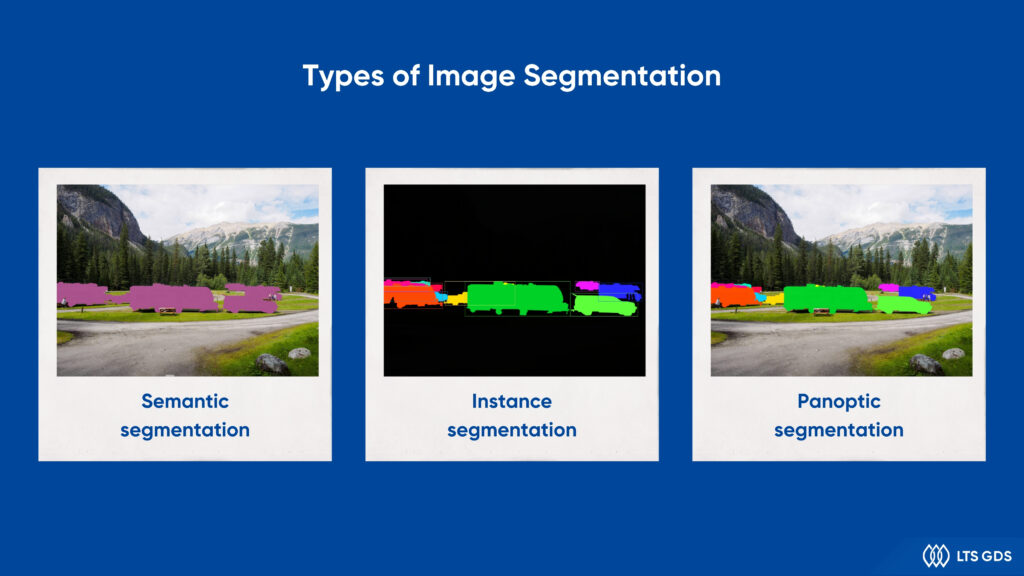
\includegraphics[width=1.0\textwidth]{images/segmentation_types_comparison.jpg}
	\captionof{figure}{So sánh ba loại phân đoạn ảnh. (Từ trái sang): Ảnh gốc, Phân đoạn Ngữ nghĩa (tất cả cừu chung một màu), Phân đoạn Thực thể (mỗi con cừu là một đối tượng riêng), và Phân đoạn Toàn cảnh (kết hợp cả hai).}
	\label{fig:segmentation_types}
\end{center}
% Keyword gợi ý: semantic instance panoptic segmentation comparison

\subsection{Phân đoạn Ngữ nghĩa: Kiến trúc Mã hóa-Giải mã và U-Net}
\label{subsec:semantic_segmentation_unet}
Bài toán phân đoạn ngữ nghĩa đòi hỏi một kiến trúc có khả năng vừa hiểu được ngữ cảnh toàn cục (để biết pixel này thuộc về "xe hơi"), vừa giữ lại được thông tin không gian chi tiết (để vẽ được đường viền chính xác của chiếc xe). Điều này đã dẫn đến sự ra đời của một họ kiến trúc cực kỳ thành công: \textbf{kiến trúc mã hóa-giải mã (encoder-decoder architecture)}.

\subsubsection{U-Net (2015): Một Cuộc cách mạng trong Ảnh Y tế}
\label{subsubsec:unet}

\textbf{U-Net} \cite{Ronneberger2015}, phát triển tại Đại học Freiburg, là mô hình kinh điển trong phân đoạn ảnh y tế, ban đầu được thiết kế cho phân đoạn tế bào trong ảnh hiển vi.

\textbf{Kiến trúc Đối xứng hình chữ U:}  
Kiến trúc U-Net có hình dạng chữ U đặc trưng, gồm hai phần chính:

\begin{description}
	\item[Nhánh Thu hẹp (Contracting Path) - Encoder:] 
	\begin{itemize}
		\item Gồm các khối tích chập $3 \times 3$ theo sau là max-pooling $2 \times 2$.
		\item Mục tiêu: giảm độ phân giải không gian, tăng số kênh đặc trưng, học các đặc trưng ngữ nghĩa trừu tượng (“what”).
		\item Mỗi bước giảm độ phân giải cũng được tăng gấp đôi số filter, giúp mạng học được các pattern phức tạp hơn.
	\end{itemize}
	
	\item[Nhánh Mở rộng (Expanding Path) - Decoder:] 
	\begin{itemize}
		\item Dùng up-sampling hoặc transposed convolution $2 \times 2$ để tăng gấp đôi kích thước feature map.
		\item Giảm số kênh, khôi phục độ phân giải không gian, học cách định vị các đặc trưng đã học được (“where”).
		\item Mỗi bước decoder kết hợp với thông tin từ encoder tương ứng nhờ skip connection.
	\end{itemize}
	
	\item[Kết nối tắt (Skip Connections):] 
	\begin{itemize}
		\item Cho phép feature map chi tiết từ encoder được truyền trực tiếp sang decoder.
		\item Giúp decoder kết hợp thông tin ngữ nghĩa bậc cao với chi tiết không gian bậc thấp.
		\item Là yếu tố chính giúp U-Net tạo mặt nạ phân đoạn vừa chính xác vừa sắc nét.
	\end{itemize}
\end{description}

\begin{mdframed}[style=infobox]
	\textbf{Trực giác của Skip Connections trong U-Net:} \\
	Encoder qua nhiều lớp pooling làm mất chi tiết không gian, trong khi decoder sau up-sampling lại có thông tin ngữ nghĩa tốt nhưng mờ về định vị. Skip connections tạo ra “đường cao tốc” cho thông tin chi tiết từ encoder, giúp decoder tổng hợp cả hai thế giới: ngữ nghĩa bậc cao + chi tiết không gian bậc thấp.
\end{mdframed}

\textbf{Hàm mất mát trong phân đoạn ảnh:}  
Để huấn luyện U-Net, thường sử dụng các hàm mất mát dựa trên pixel như \textbf{Binary Cross-Entropy (BCE)} hoặc các hàm mất mát dựa trên độ trùng khớp (overlap) như \textbf{Dice Loss}.  

\paragraph{Binary Cross-Entropy Loss:}
\begin{equation}
	\mathcal{L}_{BCE} = - \frac{1}{N} \sum_{i=1}^{N} \big[ y_i \log(\hat{y}_i) + (1 - y_i)\log(1 - \hat{y}_i) \big]
\end{equation}
với $y_i$ là nhãn ground-truth tại pixel $i$ và $\hat{y}_i$ là xác suất dự đoán.

\paragraph{Dice Loss:}  
Đo độ trùng khớp giữa mặt nạ dự đoán và ground-truth:
\begin{equation}
	\mathcal{L}_{Dice} = 1 - \frac{2 \sum_i y_i \hat{y}_i}{\sum_i y_i + \sum_i \hat{y}_i + \epsilon}
\end{equation}
với $\epsilon$ là hằng số nhỏ để tránh chia cho 0.

\textbf{Các cải tiến và mở rộng:}  
\begin{itemize}
	\item \textbf{3D U-Net:} Mở rộng cho ảnh volumetric, ví dụ MRI, CT.
	\item \textbf{Attention U-Net:} Thêm cơ chế attention để tập trung vào các vùng quan trọng.
	\item \textbf{Residual U-Net, UNet++:} Thêm residual connections hoặc nested skip connections để tăng hiệu quả học và cải thiện độ chính xác.
	\item \textbf{Ứng dụng rộng rãi:} Từ y tế (tế bào, MRI, CT) đến ảnh vệ tinh, robot, và các bài toán phân đoạn vật thể tổng quát.
\end{itemize}

\begin{center}
	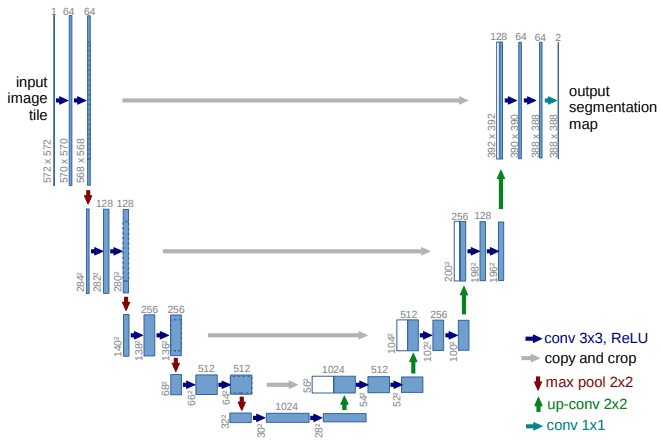
\includegraphics[width=0.9\textwidth]{images/unet_architecture_diagram.png}
	\captionof{figure}{Sơ đồ kiến trúc U-Net. Encoder bên trái học các đặc trưng ngữ nghĩa, decoder bên phải khôi phục độ phân giải không gian. Các mũi tên màu xám là skip connections quan trọng nhất.}
	\label{fig:unet_architecture}
\end{center}

\subsubsection{Các Biến thể và Hướng phát triển}
\label{subsubsec:semantic_segmentation_variants}

Thành công của U-Net đã truyền cảm hứng cho vô số các biến thể và cải tiến trong phân đoạn ảnh:

\begin{itemize}
	\item \textbf{DeepLab Family (v1–v3+)} \cite{Chen2017}: 
	\begin{itemize}
		\item Thay vì pooling để giảm độ phân giải, sử dụng \textbf{Atrous/Dilated Convolution} để mở rộng trường thụ cảm mà không làm mất chi tiết không gian.
		\item DeepLabv3+ giới thiệu \textbf{Atrous Spatial Pyramid Pooling (ASPP)}: kết hợp nhiều tỷ lệ giãn nở khác nhau, giúp mạng nắm bắt bối cảnh ở nhiều quy mô.
		\item Có khả năng xử lý các vật thể lớn nhỏ đồng thời, cải thiện độ chính xác trên ảnh y tế và ảnh tự nhiên.
	\end{itemize}
	
	\item \textbf{Attention U-Net (2018)} \cite{Oktay2018}: 
	\begin{itemize}
		\item Thêm cơ chế \textbf{Attention Gates} vào các skip connections, giúp mạng tự động tập trung vào các vùng quan trọng, giảm nhiễu từ các khu vực không liên quan.
		\item Cải thiện hiệu năng trên các bộ dữ liệu y tế phức tạp với nhiều chi tiết nhỏ.
	\end{itemize}
	
	\item \textbf{UNet++ (2018)} \cite{Zhou2018}: 
	\begin{itemize}
		\item Giới thiệu \textbf{nested skip connections} giữa encoder và decoder, giúp cải thiện khả năng gradient flow và tính chính xác khi học các chi tiết phức tạp.
		\item Tăng cường khả năng học các đặc trưng đa mức, hữu ích cho các vật thể có kích thước khác nhau.
	\end{itemize}
	
	\item \textbf{3D U-Net (2016)} \cite{Cicek2016}: 
	\begin{itemize}
		\item Mở rộng U-Net sang không gian 3D, áp dụng cho ảnh volumetric (MRI, CT).
		\item Các khối tích chập và pooling đều là 3D, giúp mạng học các đặc trưng không gian ba chiều.
	\end{itemize}
	
	\item \textbf{SegFormer (2021)} \cite{Xie2021}: 
	\begin{itemize}
		\item Kiến trúc lai \textbf{CNN + Transformer}, sử dụng Transformer Encoder phân cấp để trích xuất đặc trưng đa tỷ lệ.
		\item Decoder chỉ gồm các lớp MLP nhẹ, giảm chi phí tính toán nhưng vẫn giữ độ chính xác cao.
		\item Mang lại hiệu năng tốt trên các bộ dữ liệu lớn và đa dạng mà không cần kiến trúc phức tạp.
	\end{itemize}
	
	\item \textbf{Swin UNETR / nnFormer (2021–2022)}: 
	\begin{itemize}
		\item Sử dụng \textbf{Swin Transformer} hoặc Transformer toàn phần cho encoder, kết hợp với decoder kiểu U-Net.
		\item Xu hướng hiện nay cho các bài toán y tế: học đặc trưng toàn cục tốt hơn, xử lý các chi tiết tinh vi trong ảnh volumetric.
	\end{itemize}
	
	\item \textbf{Các xu hướng mới}: 
	\begin{itemize}
		\item Kết hợp \textbf{Attention + Multi-scale feature fusion} để tối ưu hóa thông tin ngữ nghĩa và chi tiết.
		\item Sử dụng các \textbf{loss function nâng cao}: Dice + BCE, Tversky loss, Focal loss, để cân bằng class imbalance.
		\item Biến thể lightweight: Mobile U-Net, Efficient U-Net, tối ưu cho triển khai trên edge devices.
	\end{itemize}
\end{itemize}

\textbf{Nhận xét chung:} Các biến thể này đều kế thừa ý tưởng cơ bản của U-Net (encoder–decoder với skip connections), nhưng bổ sung các cơ chế attention, multi-scale, Transformer hoặc các skip connections phức tạp hơn. Mục tiêu chung là cải thiện độ chính xác phân đoạn, khả năng học các chi tiết nhỏ, khả năng tổng quát hóa và tối ưu hóa hiệu năng tính toán.

\subsection{Phân đoạn Thực thể: Kế thừa từ Mask R-CNN và Các Biến thể}
\label{subsec:instance_segmentation_mask_rcnn}

Như đã đề cập ở phần \ref{subsubsec:cnn_based_detectors} trong mục Object Detection, \textbf{Mask R-CNN} \cite{He2017} mở rộng Faster R-CNN bằng cách thêm một nhánh Mask Head để dự đoán mặt nạ nhị phân cho từng RoI. Ở phần này, chúng ta sẽ không lặp lại kiến trúc cơ bản, mà tập trung vào các \textbf{biến thể, xu hướng và cải tiến} từ Mask R-CNN:

\begin{itemize}
	\item \textbf{Biến thể hiệu quả và nhẹ:} 
	\begin{itemize}
		\item \textbf{YOLACT, YOLACTEdge:} Biến thể single-stage của Mask R-CNN, dự đoán mask trực tiếp từ feature map, đạt tốc độ cao.
		\item \textbf{TensorMask, CondInst:} Sử dụng biểu diễn dense mask hoặc dynamic convolution, cải thiện khả năng học mask mà không cần RoIAlign phức tạp.
	\end{itemize}
	
	\item \textbf{Anchor-free Instance Segmentation:}
	\begin{itemize}
		\item \textbf{CenterMask, SOLOv2:} Dự đoán mask dựa trên các điểm tâm hoặc lưới chia ô, loại bỏ anchor, đơn giản hóa pipeline và tăng tốc độ.
		\item Xu hướng hiện nay là kết hợp anchor-free với multi-scale features để cải thiện vật thể nhỏ.
	\end{itemize}
	
	\item \textbf{Ứng dụng Transformer:}
	\begin{itemize}
		\item \textbf{Mask2Former, QueryInst:} Sử dụng cơ chế query-based attention (tương tự DETR) để học trực tiếp các đối tượng và mask, không cần RoI.
		\item Giúp thống nhất pipeline cho detection, instance segmentation, và semantic segmentation.
	\end{itemize}
	
	\item \textbf{Các cải tiến về độ chính xác và tốc độ:}
	\begin{itemize}
		\item Sử dụng \textbf{multi-scale feature fusion} để xử lý vật thể nhỏ.
		\item Loss nâng cao: Dice Loss, Focal Loss cho mask, giúp cân bằng class imbalance.
		\item Lightweight backbone và pruning để triển khai realtime trên edge devices.
	\end{itemize}
\end{itemize}

\textbf{Nhận xét:} Mask R-CNN đã đặt nền móng cho phân đoạn thực thể hiện đại. Các nghiên cứu sau này tập trung vào việc tăng tốc, loại bỏ anchor, kết hợp attention/Transformer, và cải thiện độ chính xác mask trên vật thể nhỏ hoặc khó nhận biết, đồng thời giữ pipeline end-to-end.

\subsection{Kỷ nguyên Transformer và các Mô hình Nền tảng cho Phân đoạn}
\label{subsec:transformer_foundation_models_segmentation}

Trong vài năm gần đây, phân đoạn ảnh chứng kiến một bước nhảy vọt lớn hơn cả U-Net hay Mask R-CNN: các \textbf{mô hình nền tảng (foundation models)} có khả năng phân đoạn \textit{mọi thứ}, bao gồm cả khả năng zero-shot và interactive segmentation. Các mô hình này không chỉ học để dự đoán mặt nạ, mà còn học một \textbf{không gian biểu diễn chung} (shared embedding space) cho hình ảnh và đối tượng.

\subsubsection{Segment Anything Model (SAM, 2023)}
\label{subsubsec:sam}

\textbf{Khái niệm cốt lõi:} SAM \cite{Kirillov2023} định nghĩa phân đoạn như một hàm:
\begin{equation}
	\mathcal{M}: (I, P) \mapsto \hat{M},
\end{equation}
trong đó $I$ là ảnh đầu vào, $P$ là prompt (điểm, bounding box, văn bản, mask thô), và $\hat{M} \in [0,1]^{H \times W}$ là mặt nạ dự đoán. Mục tiêu là học một mapping tổng quát, có thể áp dụng cho bất kỳ ảnh hay đối tượng nào.

\textbf{Kiến trúc chi tiết:}
\begin{itemize}
	\item \textbf{Image Encoder:} Một Vision Transformer (ViT-Huge), ánh xạ ảnh $I$ thành một tensor embedding $E_I \in \mathbb{R}^{N \times D}$, với $N = H \cdot W / p^2$ token và $D$ chiều embedding. Phép ánh xạ có thể được biểu diễn:
	\begin{equation}
		E_I = \text{ViT}(I)
	\end{equation}
	\item \textbf{Prompt Encoder:} Mỗi loại prompt $P$ được ánh xạ thành embedding $E_P \in \mathbb{R}^{L \times D}$, nơi $L$ là số token đặc trưng cho prompt (ví dụ 1 token cho click, nhiều token cho text prompt).
	\item \textbf{Mask Decoder:} Sử dụng cross-attention giữa $E_P$ và $E_I$ để học mapping phi tuyến:
	\begin{equation}
		\hat{M} = \sigma \big( \text{Decoder}(E_I, E_P) \big),
	\end{equation}
	với $\sigma$ là sigmoid, đảm bảo đầu ra là mặt nạ nhị phân xác suất.
	\item \textbf{Dữ liệu khổng lồ:} SAM được huấn luyện trên SA-1B (1.1 tỷ mặt nạ trên 11 triệu ảnh), giúp embedding $E_I$ và $E_P$ trở nên cực kỳ tổng quát.
\end{itemize}

\textbf{Tư duy nền tảng:}
\begin{itemize}
	\item Phân đoạn trở thành \textit{truy vấn (query)} thay vì dự đoán dày đặc trên toàn bộ ảnh.
	\item Tối ưu hóa end-to-end: learning objective là giảm BCE Loss cho mặt nạ:
	\begin{equation}
		\mathcal{L}_{mask} = - \frac{1}{HW} \sum_{i,j} \big[ M_{i,j} \log \hat{M}_{i,j} + (1-M_{i,j}) \log (1-\hat{M}_{i,j}) \big].
	\end{equation}
	\item Biểu diễn chung cho hình ảnh và prompt cho phép zero-shot segmentation.
\end{itemize}

\subsubsection{OneFormer (2023) và SEEM (2023)}
\label{subsubsec:oneformer_seem}

\textbf{OneFormer:} \cite{Jain2023} thống nhất các bài toán phân đoạn semantic, instance và panoptic. Key idea là \textbf{query-based Transformer}:
\begin{equation}
	\hat{M}_q = f_\theta(E_I, q),
\end{equation}
trong đó $q$ là query vector cho từng loại phân đoạn, và $f_\theta$ là Transformer decoder. Text prompt điều khiển kiểu phân đoạn.

\textbf{SEEM:} \cite{Zou2023} mở rộng SAM với multi-modal prompt:
\begin{equation}
	\hat{M} = g_\theta(E_I, E_{P_{text}}, E_{P_{point}}, E_{P_{bbox}}, E_{P_{sketch}}),
\end{equation}
với nhiều dạng embedding prompt, giúp thực hiện interactive segmentation cực kỳ linh hoạt.

\textbf{Tư duy chung:}
\begin{itemize}
	\item Học một \textbf{không gian embedding chung} cho ảnh và prompt.
	\item Sử dụng attention để gán thông tin prompt vào pixel tương ứng.
	\item Biến bài toán phân đoạn từ dự đoán pixel truyền thống thành \textbf{truy vấn và dự đoán mặt nạ dựa trên attention}, end-to-end.
\end{itemize}

\textbf{Bài học:} Kỷ nguyên Transformer trong phân đoạn không chỉ cải thiện hiệu năng, mà còn mở ra khả năng \textit{universal segmentation}, zero-shot, interactive segmentation, và nền tảng cho các mô hình multimodal.


\subsection{Kết luận}
Lĩnh vực phân đoạn ảnh đã đi một chặng đường dài, từ các kiến trúc U-Net và Mask R-CNN được huấn luyện chuyên biệt cho các tác vụ cụ thể, đến kỷ nguyên của các mô hình nền tảng như SAM. Các mô hình hiện đại không chỉ đơn thuần là các bộ "tô màu pixel"; chúng đang trở thành các công cụ lý luận thị giác, có khả năng hiểu và tương tác với thế giới hình ảnh theo cách của con người. Từ việc vẽ mặt nạ cho từng pixel, chúng ta đang tiến tới thời đại AI có thể hiểu, phân tách và mô tả từng vùng trong một cảnh vật theo yêu cầu.

\section*{Tài liệu tham khảo}
\begin{itemize}
	\item[1] Ronneberger, O., Fischer, P., \& Brox, T. (2015). U-net: Convolutional networks for biomedical image segmentation. In \textit{International Conference on Medical image computing and computer-assisted intervention (MICCAI)}. (Paper gốc giới thiệu U-Net).
	\item[2] He, K., Gkioxari, G., Dollár, P., \& Girshick, R. (2017). Mask r-cnn. In \textit{Proceedings of the IEEE international conference on computer vision (ICCV)}. (Paper gốc giới thiệu Mask R-CNN).
	\item[3] Kirillov, A., Mintun, E., Ravi, N., Tou, H., Caron, M., ... \& Girshick, R. (2023). Segment anything. \textit{arXiv preprint arXiv:2304.02643}. (Paper gốc giới thiệu Segment Anything Model - SAM).
	\item[4] Chen, L. C., Papandreou, G., Schroff, F., \& Adam, H. (2017). Rethinking atrous convolution for semantic image segmentation. \textit{arXiv preprint arXiv:1706.05587}. (Giới thiệu DeepLabv3 và Atrous Spatial Pyramid Pooling).
	\item[5] Xie, E., Wang, W., Yu, Z., Anandkumar, A., Alvarez, J. M., \& Luo, P. (2021). Segformer: Simple and efficient design for semantic segmentation with transformers. In \textit{Advances in Neural Information Processing Systems (NeurIPS)}. (Giới thiệu SegFormer).
	\item[6] Jain, J., Li, J., boosters, z., \& Carreira, J. (2023). Oneformer: One transformer to rule all segmentation tasks. \textit{Conference on Computer Vision and Pattern Recognition (CVPR)}. (Giới thiệu OneFormer).
	\item[7] Zou, X., et al. (2023). Segment everything everywhere all at once. \textit{arXiv preprint arXiv:2304.06718}. (Giới thiệu SEEM).
	\item[8] Long, J., Shelhamer, E., \& Darrell, T. (2015). Fully convolutional networks for semantic segmentation. In \textit{CVPR}. (Paper tiên phong về việc sử dụng mạng tích chập đầy đủ (FCN) cho phân đoạn ngữ nghĩa, nền tảng cho nhiều kiến trúc sau này).
\end{itemize}